\chapter{Simulation results}
\label{chap:results}

%% Experimental objectives
The objective of this chapter is to evaluate how the architectural design of an ACTS influences its ability to accurately and robustly manipulate a payload. The focus is on how different cable routing strategies, UAV attachment configurations, and ground hook placements influence the overall system performance.

A configuration is considered successful if the desired payload is reached with sufficiently small position and orientation errors, all cables are under positive tension throughout the maneuver, and the payload converges to an equilibrium without persistent oscillations. Since the tension and UAV-disposition planner (Equations from \eqref{eq:tensionPlanner} to \eqref{eq:tension-planner-relax}) solves a least-squares relaxation of the wrench-matching condition, there can be a residual between the achieved and desired payload wrench even at convergence, which is the main source of position and orientation tracking error observed in simulation. Therefore, position and orientation error are informative metrics for comparing architectures.

%% Why did you choose Stewart as the reference?
First, the classical Stewart configuration is analyzed and used as a reference architecture due to its geometric symmetry and extensive use in the literature. Moreover, its balanced geometry provides a meaningful baseline for comparing other ACTS architectures. If the reference configuration performs poorly under the developed controller, then the observed limitations may not result from the analyzed architecture, and the control strategy may be analyzed before drawing any conclusions.

The remaining experiments then investigate how modifications to the ground cable routing, UAV attachment geometry, and hook placement affect both the theoretical performance indices and the closed-loop behavior of the system. This progressive analysis makes it possible to identify which geometric features have the greatest influence on payload manipulation performance.

\section{Stewart platform baseline}
The Stewart platform configuration is used as a baseline for evaluating the proposed ACTS architectures. Its symmetric arrangement of the six ground cables provides a well-defined reference configuration against which alternative cable routings can be compared. The baseline is first examined using the static performance indices introduced in Section \ref{sec:performanceIndices}. 

%% Scenario A and B
Two desired payload poses are taken in considerations. In the first scenario, the desired payload orientation coincides with the world reference frame; while in the other scenario a non-zero desired orientation is imposed. This allows to analyze separately the rotational motions from the translation tracking.

In particular, the conditioning index, manipulability, radius of available wrench, capacity margin, and composite score are evaluated at the prescribed payload pose. These quantities provide a reference for assessing the wrench-generation capability and isotropy of the ground-cable arrangement. The complete ACTS configuration is then evaluated by incorporating the aerial cables and their actuation constraints. Finally, the resulting configuration is simulated in MuJoCo to verify the dynamic payload tracking behavior.

\subsection{Numerical verification of the baseline configuration}
This section verifies the implementation of the optimization and control algorithms by independently reconstructing the principal computation steps for a representative Stewart-platform configuration. The payload Jacobian, cable tensions, payload wrench, and UAV thrust commands are recomputed from the analytical equations derived in Chapter \ref{chap:design_modeling} and compared with the implementation. Agreement between the analytical calculations and the numerical results confirms the correctness of the implementation before comparing different ACTS architectures.

% This section verifies that the implemented optimization and control algorithms correctly reproduce the mathematical model derived in Chapters \ref{chap:design_modeling}. For one representative Stewart-platform configuration, each stage of the computation is independently reconstructed from the governing equations: cable directions are computed from the geometry, the resulting Jacobian is assembled, cable tensions are substituted to recover the payload wrench, and the required UAV thrust is recomputed from the static equilibrium equations. Agreement between these hand calculations and the implementation provides confidence that subsequent comparisons between ACTS architectures reflect architectural differences rather than implementation errors.

\subsubsection{Reference configuration}
Payload dimensions: $2.0 \times 2.0 \times 0.2$~m \\
Desired pose: $\mathbf p^*= [0.5, -0.5, 2.0]^\top$~m \\
Desired orientation: $\mathbf R^* = \mathbb{I}$ \\
Desired payload wrench: $\mathbf{w}_p^* = [0, 0, 9.81, 0, 0, 0]^\top$

\begin{table}[h]
    \centering
    \begin{tabular}{lccc}
        Attachment points       &    & Hook points & \\ \hline
        $A_4 \equiv A_5$ &  $[0.0, 1.1, 0.0]^\top$         &   $B_4 \equiv B_9$ &  $[0.5, 0.05, 1.9]^\top$          \\
        $A_6 \equiv A_7$ &  $[-0.9526, -0.55, 0.0]^\top$   &   $B_5 \equiv B_6$ &  $[-0.0237, -0.775, 1.9]^\top$    \\
        $A_8 \equiv A_9$ &  $[0.9526, -0.55, 0.0]^\top$    &   $B_7 \equiv B_8$ &  $[0.9763, -0.775, 1.9]^\top$     \\
    \end{tabular}
\end{table}

\subsubsection{Ground System Geometry}
Using Equation~\eqref{eq:cableVector}b, the ground cable directions $\mathbf u_i$ and the corresponding Jacobian are obtained as:

\begin{equation}
    \begin{aligned}
    \mathbf u_4 = [-0.2245,\ 0.4713,\ -0.8529]^\top \qquad \mathbf u_7 = [-0.7100,\ 0.0828,\ -0.6993]^\top \\
    \mathbf u_5 = [-0.0089,\ 0.7024,\ -0.7117]^\top \qquad \mathbf u_8 = [-0.0124,\ 0.1176,\ -0.9930]^\top \\
    \mathbf u_6 = [-0.4545,\ 0.1047,\ -0.8846]^\top \qquad \mathbf u_9 = [0.2215,\ -0.2937,\ -0.9299]^\top \\
    \end{aligned}
\end{equation}

\begin{equation}
\mathbf J_{p,\text{ground}} =
\begin{bmatrix}
-0.22445 & 0.47135 & -0.85291 & -0.42197 & 0.02245 & 0.12345 \\
-0.00888 & 0.70238 & -0.71175 & 0.26597 & -0.33812 & 0.33656 \\
-0.45452 & 0.10475 & -0.88456 & 0.25373 & -0.37586 & 0.29632 \\
-0.70998 & 0.08282 & -0.69934 & 0.20060 & 0.40409 & -0.52834 \\
-0.01239 & 0.11759 & -0.99298 & 0.28483 & 0.47420 & -0.47636 \\
0.22151 & -0.29365 & -0.92989 & -0.54081 & -0.02215 & -0.12183
\end{bmatrix}
\end{equation}

\subsubsection{Drone Attachment Geometry}
The UAV positions are not predefined but result from the tension-planning procedure described in Section \ref{sec:tensionPlanner}. The corresponding cable directions $\mathbf u_1, \mathbf u_2, \mathbf u_3$ are therefore extracted from a converged simulation run for this configuration rather than computed from known attachment coordinates:
\begin{equation}
    \begin{aligned}
\mathbf a_1 = [1.1020, -0.2692, 3.5972]^\top \\
\mathbf a_2 = [0.1802, -0.7553, 3.4976]^\top \\
\mathbf a_3 = [0.9397, -1.2760, 3.5192]^\top
    \end{aligned}
\end{equation}
Using Equation~\eqref{eq:cableVector}b, the resulting drone cable directions are
\begin{equation}
    \begin{aligned}
\mathbf u_1 = [0.0837, -0.0294, 0.9961]^\top \\
\mathbf u_2 = [0.1042, -0.3528, 0.9299]^\top \\
\mathbf u_3 = [0.2926, -0.1504, 0.9443]^\top
    \end{aligned}
\end{equation}
with $\lVert \mathbf a_i - \mathbf r_i \rVert \approx 1.503$~m for all three, consistent with the nominal drone
cable length of $1.5$~m and confirming the optimizer converged to a geometrically taut solution.
The corresponding drone Jacobian is
\begin{equation}
\mathbf J_{p,\text{drones}} =
\begin{bmatrix}
0.0837 & -0.0294 & 0.9961 & 0.2769 & -0.4661  & -0.0370\\
0.1042 & -0.1042 & 0.9299 & 0.2910 & 0.4533 & 0.1394 \\
0.2926 & -0.1504 & 0.9443 &  -0.5043 & 0.0293 & 0.1609\\
\end{bmatrix}
\end{equation}

\subsubsection{Cable Tensions}
For this configuration, the optimizer returns

\begin{equation}
\begin{aligned}
\boldsymbol{\tau}_{\text{UAV}} &= \begin{bmatrix}
13.697 & 11.155 & 14.415 \end{bmatrix}^\top~\text{N} \\
\boldsymbol{\tau}_{\text{ground}} &= \begin{bmatrix}
    5.5 & 5.5 & 5.50007894 & 5.5 & 5.5000916 & 5.5000083
\end{bmatrix}^\top~\text{N}
\end{aligned}
\end{equation}

All six ground tensions lie close to $\tau_{\min}=5.5$ N. This is not indicative of a wrench-singular configuration: since the desired wrench is almost entirely vertical, the UAVs provide most of the lifting force while the Stewart cables primarily stabilize the payload orientation and prevent lateral motion. As a result, the optimizer drives the ground tensions toward their minimum admissible values, maintaining taut cables while minimizing unnecessary internal forces. This observation is confirmed by the capacity margins ($\gamma = 10.46403$, Table \ref{tab:stewart_comparative}), highly positive compared to the negative value obtained when using the minimal tension strategy explained in Section \ref{sec:allocationStrategies}.

\subsubsection{Payload Wrench Verification}
Combining $\mathbf J_{p,\text{drones}}$ and $J_{p,\text{ground}}$ into the full Jacobian $\mathbf J_p$ and evaluating $\mathbf W_p = \mathbf J_p\, \boldsymbol{\tau}$ with the tensions above:
\begin{equation}
\mathbf W_p = \mathbf J_p\, \boldsymbol{\tau} =
\begin{bmatrix} -0.0023 \\ 0.0018 \\ 9.8110 \\ -0.0003 \\ -0.0001 \\ -0.0009 \end{bmatrix},
\qquad
W_p^* =
\begin{bmatrix} -0.0158 \\ 0.0180 \\ 9.7341 \\ -0.0022 \\ 0.0019 \\ -0.0151 \end{bmatrix}.
\end{equation}

All six components match to within $0.08$ in force units and $0.015$ in moment units. The residual remains small, confirming that the optimizer reproduces the desired wrench within the prescribed tolerance.

\subsubsection{Required Drone Thrust}
Under the steady-state assumption $\mathbf p^* = \mathbf p$, $\dot{\mathbf p}^* = \dot{\mathbf p} = \mathbf 0$,
Eq.~\eqref{eq:drone-disposition} reduces to $F_{prop,i} = \tau_i \mathbf u_i + m_i g\, \mathbf e_3$, giving the hand-computed thrust magnitudes
\begin{equation}
T_1 = 33.29~\text{N}, \qquad T_2 = 30.27~\text{N}, \qquad T_3 = 33.57~\text{N}.
\end{equation}
The controller-computed thrust commands for the same converged pose are $33.2793$, $30.2683$, and $33.5657$~N respectively, matching the hand-computed values to within numerical precision and confirming the correct implementation of Eq. \eqref{eq:drone-disposition}.

\subsubsection{Discussion}
The numerical verification confirms the correctness of both the optimization and control implementations. These results provide confidence that the subsequent comparison of ACTS architectures reflects differences in the robot configurations rather than implementation errors.

\subsection{Comparison between tension allocation strategies}
\label{sec:allocationStrategies}
As mentioned in Section \ref{sec:highlevelarchitecture}, we evaluate two distinct tension allocation strategies:
\begin{itemize}
    \item Minimal tension strategy, in which a minimum cable tension is imposed to each cable tension such that $\|\tau_i \| = \tau_{min}$.
    \item Optimal tension strategy, in which cable tensions are determined by the quadratic optimization problem in Equation \eqref{eq:tension-planner-relax}
\end{itemize}

The performance indices and tracking errors under both strategies across two operational scenarios are summarized in Table \ref{tab:stewart_comparative}.


The minimal tension strategy has negative consequences on the system's robustness. By locking all cable tensions to their absolute lowest limit ($\tau_{\min}$), the range of available tension choices shrinks to a single point. As a result, the controller loses its ability to adjust forces, reducing the payload's Available Wrench Set (AWS) to just a single fixed outcome. \cite{yang_robust_2025}
% Even though being faster, the minimal tension strategy has negative consequences on the system's robustness. Fixing the tension vector to its lower limit $\tau_{\min}$ collapses the tension space from an $N$-orthotope $[\tau_{\min}, \tau_{\max}]^N$ to a single point, which linearly maps through the wrench matrix $W$ to degenerate the Available Wrench Set (AWS) into a single point \cite{yang_robust_2025}. 
As a result, any deviation of the desired payload wrench $W_p^*$ from this single point results in a negative capacity margin (as seen in Scenario A where $\gamma = -0.19343$). This indicates that the system is theoretically incapable of resisting external disturbances or maintaining equilibrium without violating the tension constraints.


\begin{table}[htbp]
\centering
\small
\begin{threeparttable}
\begin{tabular}{rcccc}
\toprule
 & \multicolumn{2}{c}{\textbf{Scenario A}} & \multicolumn{2}{c}{\textbf{Scenario B}} \\
\cmidrule(lr){2-3} \cmidrule(lr){4-5}
\textbf{Metric / Parameter} & $\tau_{\text{min}}$ & $\tau_{\text{opt}}$ & $\tau_{\text{min}}$ & $\tau_{\text{opt}}$ \\ 
\midrule
Desired Position & \multicolumn{2}{c}{$[0.5, -0.5, 2.0]^\top$} & \multicolumn{2}{c}{$[0.5, -0.5, 2.0]^\top$} \\
Desired Orientation & \multicolumn{2}{c}{$[1.0, 0.0, 0.0, 0.0]^\top$} & \multicolumn{2}{c}{$[1.0, 0.1, -0.1, 0.1]^\top$} \\
\midrule
$\nu$  & 0.10259 & 0.09617 & 0.07052 & 0.05550 \\
$w$ & 0.47775 & 0.43700 & 0.31471 & 0.24108 \\
$rAW_{force}$  & 49.29711 & 47.90399 & 52.21278 & 53.22707 \\
$\gamma$ & -0.19343 & 10.46403 & -3.83256 & 2.65386 \\
$\zeta$  &  0.90998 & 0.76401 & 0.90998 & 0.75072 \\
$N$ & 17.35180 & 20.62849 & 17.64446 & 19.42488 \\
\midrule
Position Error & 0.00201 & 0.00284 & 0.00187 & 0.00262 \\
Orientation Error & 0.00121 & 0.00209 & 0.00379 & 0.00385 \\
\bottomrule
\end{tabular}
\caption{Comparative performance indices and tracking errors for Stewart baseline configuration across Scenarios A and B.}
\label{tab:stewart_comparative}

\end{threeparttable}
\end{table}


Switching to the optimal tension allocation, allows the cable tensions to vary dynamically between $\tau_{min}$ and $\tau_{max}$. As a result, the radius of the available wrench rAW increases and the capacity margin takes on a positive value ($\gamma = 10.46403$). Thus, also the composite score increases. Differently, changing the tension allocation algorithm has no effect on the conditioning index or manipulability because they are kinematic metrics that only depend on the platform's geometric position.

An ideal ACTS architecture should remain far from singular configurations, generate payload wrenches efficiently in every direction, and maintain sufficient redundancy to accommodate disturbances while respecting cable tension limits. Consequently, all the considered performance indices should be as big as possible. The considerations from now on will be done using the optimal tension strategy.

% \noindent On the other hand, it is worth to notice that, since the objective function does not contain any state-tracking terms, this optimizer does not directly minimize the payload's real-time position or orientation tracking errors. 
% Because of this, a spatial configuration that yields globally minimal propulsion effort does not guarantee a minimum in tracking error.

Although the Stewart configuration exhibits good overall performance and provides an excellent reference architecture, the proposed ACTS differs from a classical Stewart platform because the UAV cables can be connected to the payload in several different ways. Moreover, different ground cable routings may further improve specific performance aspects such as stability, wrench generation capability, or robustness. For these reasons, the Stewart configuration is adopted as a baseline against which all alternative architectures are compared. 


\begin{figure}
    \centering
    \begin{subfigure}{0.8\linewidth}
        \centering
        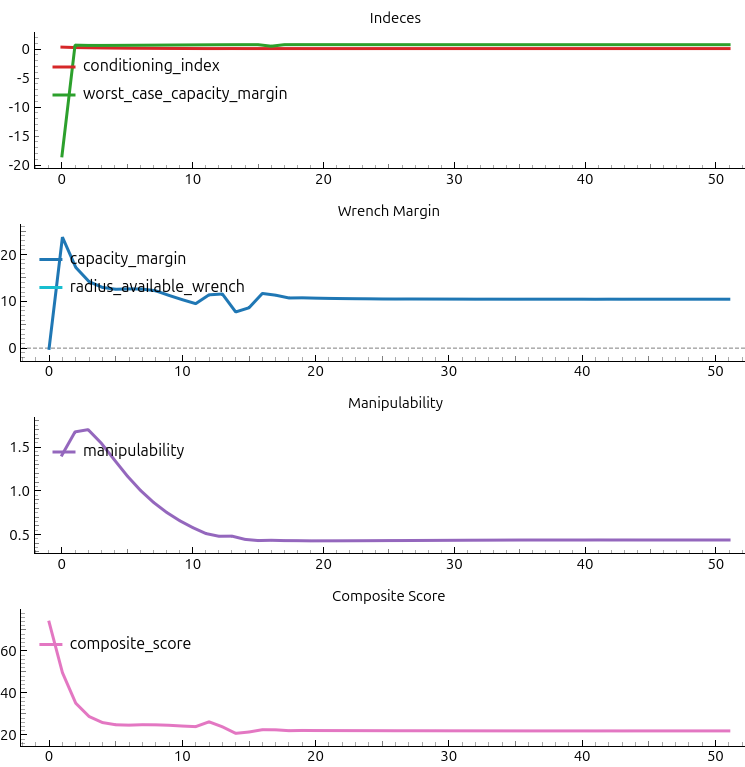
\includegraphics[width=\linewidth]{images/simulation_graphs/acts_stewart_tau_optimal_0.5--0.5-2.0_1.0-0.0-0.0-0.0_indices.png}
        \caption{Performance indices}
        \label{fig:performanceIdxATauOpt}
    \end{subfigure}
    \hfill
    \begin{subfigure}{0.8\linewidth}
        \centering
        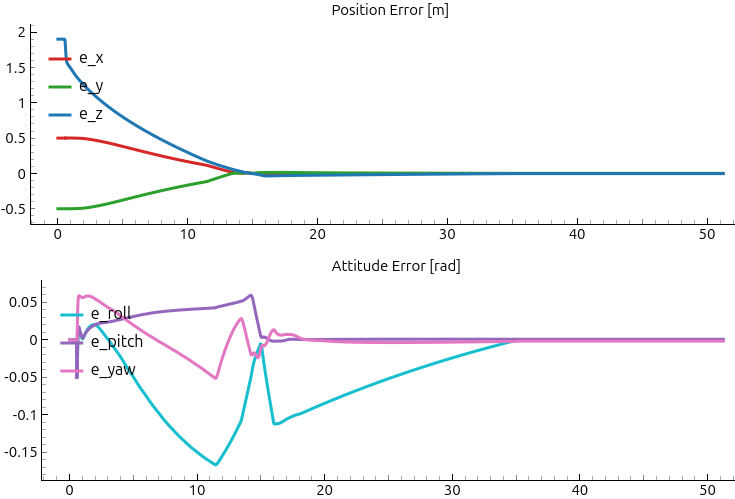
\includegraphics[width=\linewidth]{images/simulation_graphs/acts_stewart_tau_optimal_0.5--0.5-2.0_1.0-0.0-0.0-0.0_errors.png}
        \caption{Pose error}
        \label{fig:errorTauOpt}
    \end{subfigure}
    \caption{Trend of performance indices and pose error in the simulation with optimal tension strategy for $\mathbf p^* = [0.5, -0.5, 2.0]^\top$ and $\mathbf R = \mathbb{I}$}
    \label{fig:tauopt}
\end{figure}


\begin{figure}
    \centering
    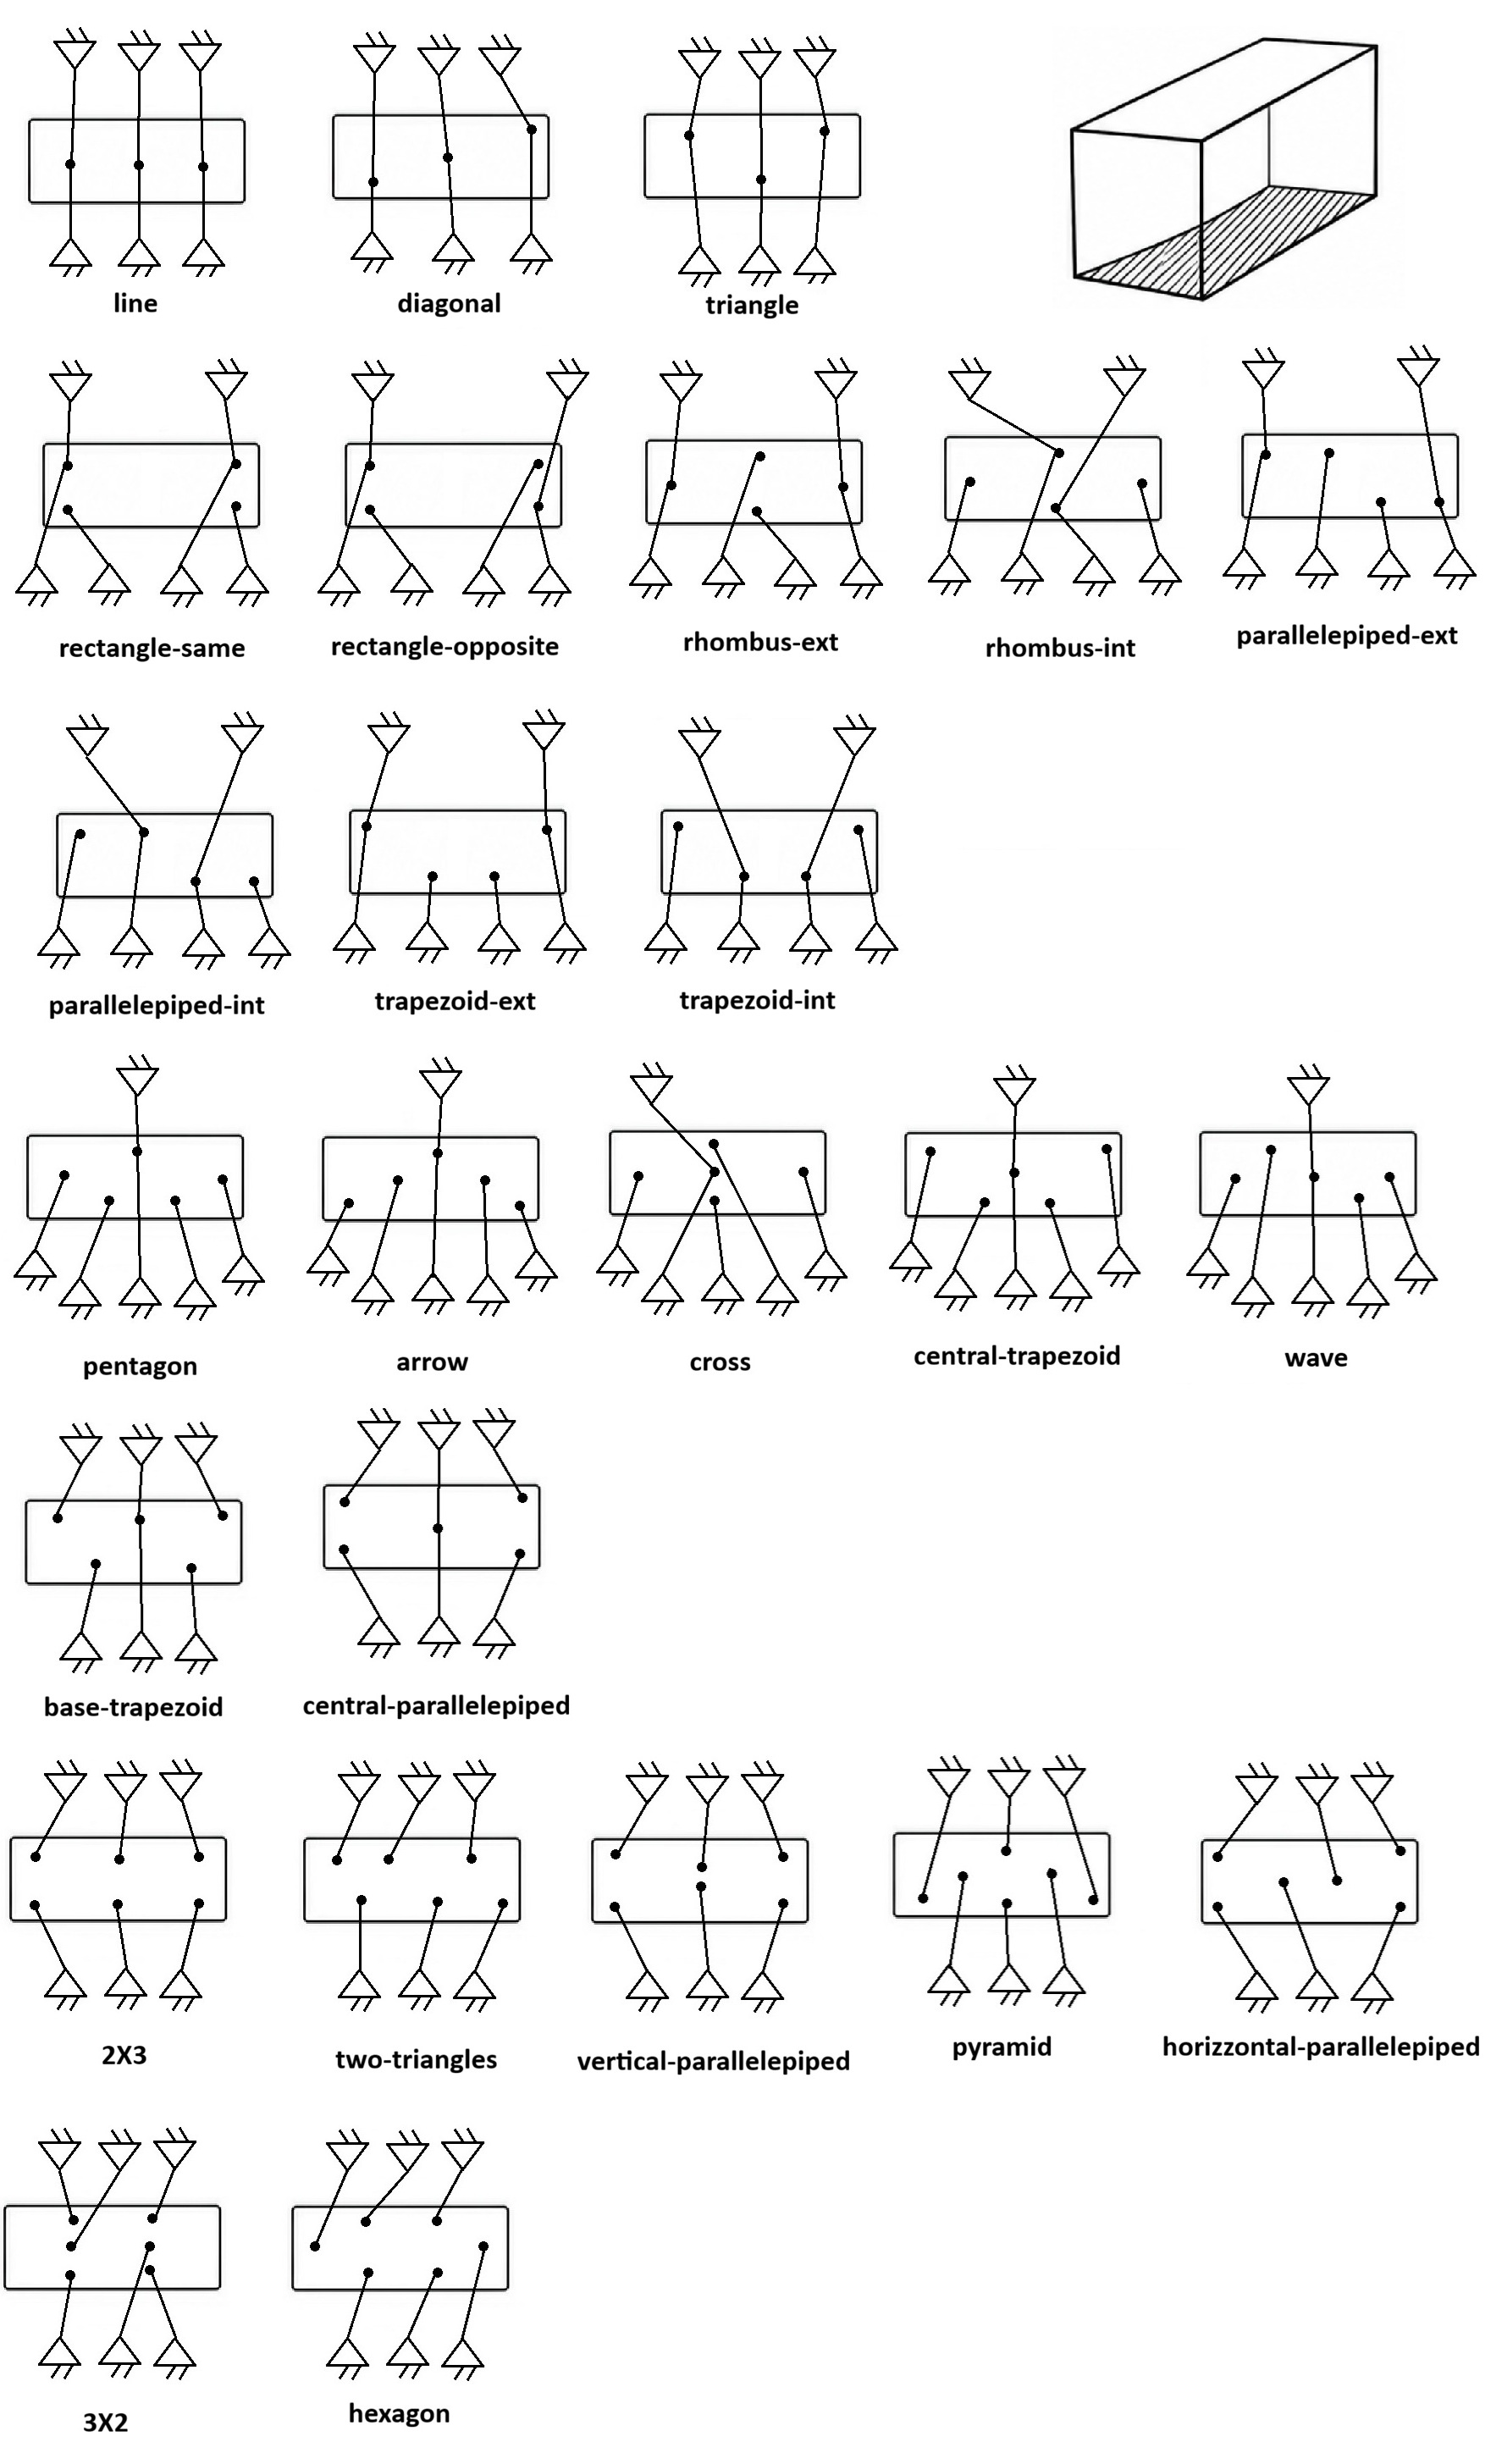
\includegraphics[width=0.65\linewidth]{images/6_ugv_config.jpeg}
    \caption{Possible 6 UGVs connections}
    \label{fig:6ugvsConnections}
\end{figure}

\begin{figure}
    \centering
    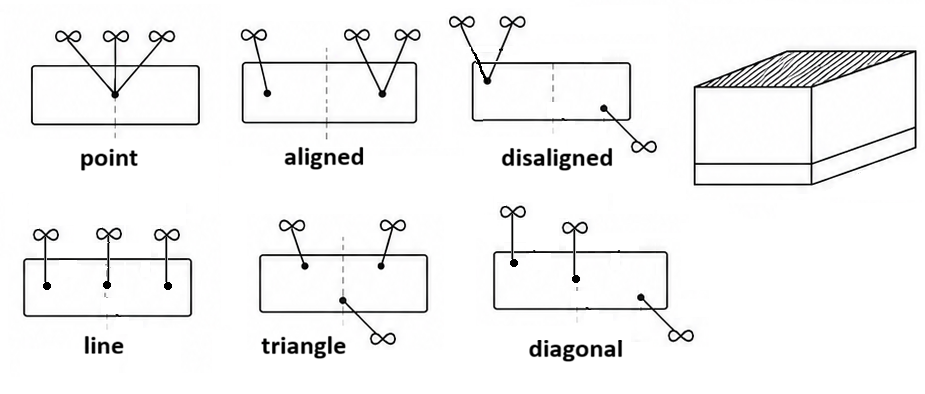
\includegraphics[width=0.65\linewidth]{images/3_uav_config.png}
    \caption{Possible 3 UAVs connection with one cable}
    \label{fig:3uavsConnections}
\end{figure}

\section{Statistical tests}
\label{sec:statisticTest}

Every configuration is assessed on the same set of poses, making them comparable on the basis of the result obtained. Particularly, the performance of each robot configuration was evaluated using a set of continuous and binary performance metrics extracted from the simulations. 

Continuous metrics were analyzed using the Friedman test, whereas binary metrics were analyzed using Cochran's Q test. For metrics exhibiting a statistically significant omnibus result, post-hoc comparisons against the reference configuration were performed using paired Wilcoxon signed-rank tests for continuous variables and McNemar's exact tests for binary variables.

Since multiple statistical tests were performed, corrections were applied to reduce the probability of false-positive results. The Benjamini-Hochberg false discovery rate correction was applied to the omnibus tests, while Holm's correction was applied to the post-hoc comparisons. 

Statistical significance was assessed using a significance level of $\alpha = 0.05$. A detailed description of the adopted statistical methods is provided in Appendix \ref{app:statistics}.


\section{Ground cable routing}

Once the controller has been validated using the Stewart baseline, we can proceed to consider different ways to connect six ground cables to the platform (Figure \ref{fig:6ugvsConnections}) and the drone (Figure \ref{fig:3uavsConnections}). The same ground configuration hook-anchor can change the system's stability based on which hook is connected to which anchor point on the ground.
%% Why we choose the triangle for the UAVs configuration?
Therefore, we will start considering the drone attachment configuration as fixed to the triangular arrangement and vary only the routing of the six ground cables. This specific UAV configuration is chosen because it provides a symmetric distribution of the three drones around the payload. This approach allows one to isolate the influence of the ground cable routing and attribute differences in performance solely to the ground architecture. Finally, in Section \ref{sec:dronehook}, the impact of various UAV attachment geometries is examined independently.

%% How the code work, how a given cable routing has been found
Focusing on the ground cable routing, there are at most $6! = 720$ physically distinct valid ways to route the six ground cables. Scoring an architecture using only one arbitrarily chosen routing raise the question on how lucky the routing choice was and how good the architecture actually is. Therefore, implementing the selection strategy explained in Section \ref{sec:selection_strategy} is essential to make a guided choice and conclusions on the results.

\subsection{Ground screening}
\label{sec:ground_screening}
The pre-screening results are shown in Table \ref{tab:prescreening_feasibility} and Table \ref{tab:prescreening_index}, where ground cable routings were tested over 10 different poses.
Any routing that violates either WCC or IFC at any tested pose is removed, as it was explained deeply in Section \ref{sec:selection_strategy}.  For this reason, the WCC and IFC counts in Table \ref{tab:prescreening_feasibility} are per-routing failures, while the WFC count is not directly comparable, since it represents the total number of pose-level failures accumulated across all candidate routings. The WFC is the main cause of rejection, which means that many routings are still kinematically feasible, but they cannot produce the required wrench while keeping the cable tensions within the allowed range. The WCC failures are relatively few, indicating that rank deficiency is less common than tension infeasibility. IFC failures are only  caused by cable-cable interference, and not by exit-angle violations.

The quality of the selected routing is evaluated through four complementary metrics. The smallest singular value, $\sigma_{\min}$, measures the distance from singular configurations, while the conditioning index $\nu$ evaluates the isotropy of the wrench generation capability. Manipulability quantifies the overall size of the achievable wrench space, whereas $d_{\min}$ characterizes the minimum cable-to-cable clearance over all tested poses.

Table \ref{tab:prescreening_index} shows how no single architecture simultaneously maximizes every performance metric. The two-triangles-vertical-parallelepiped configuration provides the largest minimum singular value and the best conditioning index, indicating the greatest robustness against singular configurations. In contrast, the rectangle-opposite-2x3 architecture performs the highest manipulability, suggesting a larger overall wrench capability. Finally, the parallelepiped-int-2x3 layout provides the largest minimum cable clearance, reducing the likelihood of cable interference. These results highlight the trade-off between kinematic robustness, wrench capability, and geometric clearance.

\begin{table}[htbp]
\centering
\resizebox{\linewidth}{!}{
\begin{tabular}{lcccc}
\toprule
\textbf{Layout} & \textbf{WCC} & \textbf{WFC} & \textbf{IFC} & \\
\textbf{(Payload -- Ground)} & \textbf{Failures} & \textbf{Failures} & \textbf{Failures} & \textbf{Feasible} \\
\midrule
two-triangles -- vertical-parallelepiped    & 64 & 2538 & 507 & \checkmark \\
rectangle-opposite -- 2X3                    & 72 & 146  & 94  & \checkmark \\
parallelepiped-int -- 2X3                   & 52 & 340  & 102 & \checkmark \\
parallelepiped-ext -- horizzontal-parallelepiped & 24 & 630 & 116 & \checkmark \\
central-trapezoid -- horizzontal-parallelepiped  & 16 & 1186 & 255 & \checkmark \\
\bottomrule
\end{tabular}
}
\caption{Pre-screening feasibility of cable-routing architectures}
\label{tab:prescreening_feasibility}
\end{table}

\begin{table}[htbp]
\centering
\begin{threeparttable}

\begin{tabular}{lcccc}
\toprule
\textbf{Layout (Payload -- Ground)} & $\sigma_{\min}$ \tnote{a} & $\nu$ \tnote{b} & $w$ \tnote{c}& $d_{\min}$ \tnote{d}  \\
\midrule
two-triangles -- vertical-parallelepiped    & 0.1911 & 0.0797 & 0.0450       & 0.0638 \\
rectangle-opposite -- 2X3                    & 0.1875 & 0.0786 & 0.0957      & 0.2027 \\
parallelepiped-int -- 2X3                   & 0.1892 & 0.0784 & 0.0344       & 0.3213 \\
parallelepiped-ext -- horizzontal-parallelepiped & 0.1825 & 0.0750 & 0.0302  & 0.1921 \\
central-trapezoid -- horizzontal-parallelepiped  & 0.1676 & 0.0696 & 0.0290  & 0.1452 \\
\bottomrule
\end{tabular}
\caption{Best routing quality across feasible architectures}
\label{tab:prescreening_index}

\begin{tablenotes}
\footnotesize
\item[a] $\sigma_{\min}$ = smallest singular value of the payload Jacobian.
\item[b] $\nu$ = conditioning index (Eq. \ref{eq:conditioning_index})
\item[c] $w$ = manipulability (Eq. \ref{eq:manipulability})
\item[d] $d_{\min}$ = minimum cable-to-cable clearance of the selected routing over all tested poses.
\end{tablenotes}
\end{threeparttable}
\end{table}


\todo[inline]{Talk about triangle-triangle combination why it does not pass the pre-screening?}

Notice something very odd. It never even reached WCC/WFC/IFC failures. This suggests the algorithm never found a routing to evaluate, or the architecture was rejected before the screening loop. That is not something you can conclude from the tables.

I would first verify the code. If it is indeed skipped because: payload layout equals ground layout, or there are only six identical permutations, then discuss that.

% This is the result triangle-triangle
% pay_layout	gnd_layout	n_routings_checked	n_poses_checked	feasible	n_wcc_fail	n_wfc_fail	n_ifc_fail	n_ifc_fail_cable_cable	n_ifc_fail_exit_angle	wfc_fail_residual_min	wfc_fail_residual_median	wfc_fail_residual_max	wfc_fail_residual_force_median	wfc_fail_residual_moment_median	wfc_fail_residual_force_lateral_median	wfc_fail_residual_force_vertical_median	n_wfc_verify_attempted	n_wfc_verify_rescued	conditioning_index	manipulability	sigma_min	sigma_max	rank_ok	wfc_ok	max_wfc_residual	max_wfc_residual_force	max_wfc_residual_moment	ifc_ok	min_cable_cable_dist	min_exit_angle_margin	wfc_rescued_by_reposition	best_routing
% triangle	triangle	6	10	False	0	0	0	0	0								0	0	



\subsection{Simulation run}
%% How and why the results before simulation and after simulation differ?
The theoretical indices evaluate the geometric and static properties of a cable routing. They define configurations close to kinematic or wrench singularities, and they classify architectures based on their ability to generate payload wrenches. However, they cannot predict the transient response of the closed-loop system. Dynamic effects such as payload inertia and load redistribution are only captured by simulation. Therefore, while poor theoretical indices almost always indicate poor dynamic performance, the opposite is not necessarily true: a routing with good static indices may still have oscillations or bad tracking.

For each configuration derived in the previous step, a simulation is run over 60 different poses (shown in Figure \ref{fig:test_poses}), and conclusions are drawn. Additionally, extra simulations have been run to test specific ground cable routing and see if they lead us to further conclusions. Table \ref{tab:architecture_ranking} summarizes the results of the dynamic simulations for the candidate architectures selected during the pre-screening. The objective is to evaluate whether the theoretical metrics introduced previously are consistent with the observed closed-loop behavior. In particular, the simulations assess pose reachability, cable rubbing and numerical stability over the set of 60 testing poses. Each indicator is ranked from 1 to 5, where lower values correspond to better overall performance.


\begin{figure}
    \centering
    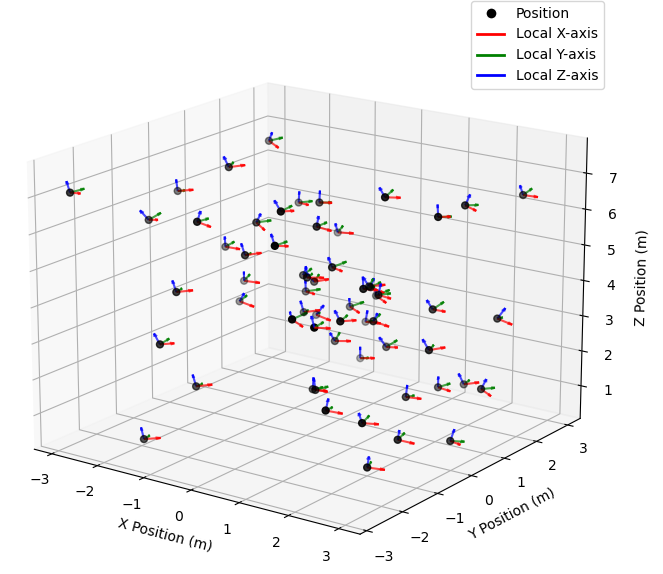
\includegraphics[width=0.65\linewidth]{images/testing_poses.png}
    \caption{Testing poses}
    \label{fig:test_poses}
\end{figure}


\begin{table}[htbp]
\centering
\begin{threeparttable}
\resizebox{\linewidth}{!}{
\begin{tabular}{l c c c c c c}
\toprule
\textbf{Architecture} & $\nu$ & $w$ & $N$ & \textbf{Pose Reach} & \textbf{Cable Rub} & \textbf{Instab.} \\
\midrule
rectangle-opposite-2x3 & 0.1246 (1) & 1.0459 (1) & 8.9142 (1) & 0.5833 (5) & 0.9333 (6) & 0.0500 (2) \\
parallel-int-2x3 & 0.0997 (4) & 0.4536 (4) & 6.7857 (2) & 0.7500 (1) & 0.4667 (3) & 0.0500 (2) \\
two-triangles-vertical-parallel & 0.1107 (3) & 0.4907 (3) & 5.9310 (3) & 0.6667 (3) & 0.9167 (5) & 0.0667 (5) \\
parallel-ext-horiz-parallel & 0.1210 (2) & 0.7770 (2) & 5.8649 (4) & 0.5333 (6) & 0.4500 (2) & 0.0500 (2) \\
acts\_stewart & 0.0533 (6) & 0.1054 (6) & 5.5706 (5) & 0.6500 (4) & 0.3167 (1) & 0.0833 (6) \\
central-trapezoid-horiz-parallel & 0.0803 (5) & 0.2099 (5) & 4.8839 (6) & 0.7333 (2) & 0.6333 (4) & 0.0333 (1) \\
\bottomrule
\end{tabular}
}
\caption{Static and dynamic performance indices for the six candidate architectures, with rank (1 = best, 6 = worst) shown in parentheses.}
\label{tab:architecture_ranking}
\begin{tablenotes}
\footnotesize
\item $\nu$ = conditioning index; $w$ = manipulability; $N$ = composite score; 
\item Pose Reach = fraction of trials reaching the target pose; 
\item Cable Rub = fraction of trials with cable rubbing; 
\item Instab. = \texttt{simulation\_unstable} rate. 
\end{tablenotes}
\end{threeparttable}
\end{table}


\todo[inline]{What does the table tells us about?}
For instance, the rectangle-opposite-2x3 architecture achieves the highest conditioning index and manipulability, yet exhibits the lowest pose reachability and the highest cable rubbing rate. Conversely, the parallelepiped-int-2x3 and central-trapezoid-horizontal-parallelepiped architectures provide better dynamic performance despite lower theoretical rankings. These results indicate that geometric quality alone is insufficient to characterize the overall behavior of the system, as dynamic effects such as payload inertia, cable force redistribution, and controller interaction become dominant during motion. The ACTS Stewart platform serves as a baseline reference, illustrating how the hybrid cable-driven architectures compare against the conventional parallel manipulator. Overall, the simulations validate the role of the pre-screening in eliminating infeasible routings while demonstrating the necessity of dynamic simulation for selecting the most suitable architecture.

\todo[inline]{How the results before simulation and after simulation differ?}

The dynamic simulations reveal that the theoretical performance indices alone do not fully predict the closed-loop behaviour of the system. The rectangle-opposite-2x3 architecture, which achieves the highest conditioning index and manipulability, exhibits the lowest pose reachability and one of the highest cable rubbing rates. Conversely, the parallelepiped-int-2x3 architecture, despite a lower conditioning index and manipulability, achieves the highest pose reachability while maintaining moderate cable interference. Similarly, the central-trapezoid-horizontal-parallelepiped architecture, which ranks lowest in the theoretical indices among the cable-driven configurations, presents the lowest instability rate. These observations indicate that the static metrics are effective for identifying geometrically favourable routings and avoiding singular configurations, but they do not account for dynamic effects such as payload inertia, force redistribution between cables, and the interaction with the controller.

Supplementary simulations have been run on configurations realized manually, rather than selected through a systematic search.

\todo[inline]{Does this give us additional results?}

The supplementary manually designed configurations further demonstrate that the cable routing itself has a significant influence on the dynamic behavior, even when the underlying payload and ground geometries remain unchanged. Architectures sharing the same layouts but employing different cable assignments exhibit noticeable differences in pose reachability, cable rubbing and instability.

Overall, the manually selected routings do not consistently outperform those obtained through the systematic screening procedure. This suggests that manually identifying a suitable routing based solely on geometric intuition is difficult, whereas the proposed screening strategy provides a more reliable and reproducible means of selecting high-quality candidate routings for subsequent dynamic evaluation.

\begin{table}[htbp]
\centering
\begin{threeparttable}
\resizebox{\linewidth}{!}{
\begin{tabular}{lcccccc}
\toprule
\textbf{Architecture} & $\nu$ & $w$ & $N$ & \textbf{Pose Reach} & \textbf{Cable Rub} & \textbf{Instab.} \\
\midrule
rect-same--rect-opposite & 0.1077 (2) & 9.1356 (1) & 9.1356 (1) & 0.6167 (5) & 1.0000 (4) & 0.2500 (3)\\
2X3--rect-same & 0.1226 (1) & 8.5115 (2) & 8.5115 (2) & 0.7000 (3) & 1.0000 (4) & 0.4833 (5) \\
horiz-parall.--horiz-parall.-3 & 0.0647 (3) & 6.6252 (3) & 6.6252 (3) & 0.7833 (1) & 0.4000 (1) & 0.0667 (1) \\
horiz-parall.--horiz-parall. & 0.0645 (4) & 6.5651 (4) & 6.5651 (4) & 0.7167 (2) & 1.0000 (4) & 0.2500 (3)\\
rect-opposite--2X3-2 & 0.1126 (5) & 6.4080 (5) & 6.4080 (5) & 0.5667 (4) & 1.0000 (4) & 0.1667 (2) \\
\bottomrule
\end{tabular}
}
\caption{Top five manual architectures}
\label{tab:architecture_ranking_manual}

\end{threeparttable}
\end{table}

\subsection{Analysis of Specific configurations}
\subsubsection{Degenerative ground configurations - Line and Diagonal}
\label{sec:degenerativeConfigurationa}
The exhaustive screening consistently rejects the line and diagonal ground-routing configurations. This result is expected, as in these layouts several cable directions become nearly coplanar or aligned, resulting in cable arrangements that are close to kinematic singularities. Consequently, the cable system can no longer generate a full six-dimensional wrench space. This result could have also been explained geometrically. In the line configuration, cable attachments lie along a single axis, which limits the system's ability to generate forces and torques in directions perpendicular to that line. Similarly, the diagonal configuration introduces a strong directional bias along the axis on which the cable attachments are positioned.

Simulation results using hand-crafted configurations confirm this conclusion: line-based and diagonal-based ground cable layouts never rank among the highest-performing architectures in terms of composite score. The drop in performance becomes particularly pronounced when both the payload and the ground attachments are arranged in a one-dimensional configuration. In such cases, the desired pose is achieved less than half the time, like in the line-line-triangle configuration that succeeds only 40\% of the time. Success rates nearly double when at least one attachment expands into two dimensions, as seen in line-pentagon-triangle (56.67\%) or line-hexagon-triangle (76.67\%).

\subsubsection{Configuration two-triangles--vertical-parallelepiped--triangle}

two-triangles-vertical-parallelepiped has the largest $\sigma_{min}$, it also has the largest conditioning index, but it has lower manipulability than rectangle-opposite. This is nice because it illustrates that: manipulability measures the overall volume of the wrench ellipsoid, whereas $\sigma_{min}$ measures the worst-case direction. So an architecture can have: slightly smaller manipulability, but a larger $\sigma_{min}$, meaning it is more isotropic and farther from singularity, even if its total wrench capability is not maximal.

The simulation results further show that neither property alone determines the dynamic performance. Although the two-triangles-vertical-parallelepiped architecture provides the largest $\sigma_{\min}$, indicating the greatest robustness against singular configurations, it does not achieve the best closed-loop performance. Likewise, the rectangle-opposite-2x3 architecture, which maximizes manipulability, performs poorly in terms of pose reachability. Therefore, $\sigma_{\min}$ and manipulability should be interpreted as complementary geometric indicators rather than direct predictors of dynamic behavior.


\todo[inline]{Other combinations that give interesting results?}
Overall, the simulation results indicate that no single architecture simultaneously optimizes every performance metric. The rectangle-opposite-2x3 architecture maximizes the theoretical indices, whereas the central-trapezoid-horizontal-parallelepiped architecture provides the highest numerical stability. The parallelepiped-int-2x3 architecture, however, offers the best overall compromise by combining the highest pose reachability with low instability and acceptable cable rubbing. Relative to the ACTS Stewart baseline, it demonstrates that the proposed cable-driven architecture can achieve comparable closed-loop performance while satisfying the additional routing constraints inherent to the hybrid system.
\section{Ground anchor placement}
\label{sec:ground-placement}
The influence of the ground-anchor spacing was evaluated by comparing three geometrically similar datasets in which the ground attachment locations were uniformly scaled while preserving the same cable-routing topologies. The comparison was restricted to the triangle-UAV configurations to isolate the effect of anchor placement from that of cable routing.

Increasing the distance between the ground anchors is expected to improve the robot's mechanical performance. A larger anchor footprint increases the moment arm between the payload and the cable attachment points, allowing the cables to generate larger restoring moments and a wider achievable wrench set. Consequently, higher wrench quality, better conditioning, and improved tracking performance are expected.

The complete numerical results for all evaluated metrics, workspace sizes, and platform configurations are reported in Appendix \ref{app:full_results}. Tables \ref{tab:metrics_part1} and~\ref{tab:metrics_part2} provide the complete metric values together with the statistical significance of each comparison relative to the reference \texttt{acts\_stewart} configuration.

\subsection{Results with reduced anchor spread}
Reducing the anchor spacing consistently degrades the performance of all alternative architectures. Static performance indicators (Table \ref{tab:metrics_part1}), including the capacity margin, manipulability, radius of available force, and conditioning index, decrease across almost every configuration. Likewise, cable rubbing becomes more frequent as the anchors are brought closer together, indicating that the cable directions become increasingly parallel and clearance between neighbouring cables is reduced.

The effect is particularly evident in the task-level metrics (Table \ref{tab:metrics_part2}). The pose reached metric shows the clearest deterioration: whereas the reference Stewart configuration successfully reaches 65\% of the target poses, all compressed alternatives achieve only 35-60\%. This difference is statistically significant ($p=0.0001$) and is reflected in the number of unreached poses, which increases from 10/60 in the nominal dataset to 15/60 in the reduced-scale dataset.

\subsection{Results with increased anchor spread}

Increasing the anchor spacing produces the opposite trend. Every static performance metric improves, with higher capacity margins, larger radii of available force, better conditioning indices, and increased manipulability across all evaluated architectures. Position and orientation tracking errors also decrease for nearly every routing, demonstrating that the improved static properties translate into better closed-loop performance.

The wider anchor distribution also improves task completion. Only three of the sixty target poses remain unreachable, compared with ten in the nominal configuration and fifteen in the reduced-scale configuration (Table \ref{tab:reachposeSize}). Interestingly, the overall difference in pose completion between routing topologies is no longer statistically significant ($p=0.069$). This suggests that, once the anchor spread is sufficiently large, the system operates well within its feasible wrench region and the choice of cable routing becomes considerably less critical.

One notable exception is the \texttt{central-trapezoid-horizontal-parallelepiped} routing, which exhibits increased position and orientation errors despite improvements in all static indices. This behavior mirrors the discrepancy between static performance measures and dynamic tracking discussed previously, indicating that favorable wrench metrics alone do not necessarily guarantee improved closed-loop accuracy.

\subsection{Considerations on the anchor spacing}
The experimental results consistently support selecting the largest feasible ground-anchor footprint. Compared with the nominal and reduced configurations, the larger footprint provides superior composite performance, larger wrench margins, better conditioning, lower tracking errors, and substantially fewer unreached poses. Furthermore, it is the only tested scale for which the routing topology no longer has a statistically significant influence on pose completion, indicating increased robustness to architectural choices.

The improvement in reachability is also spatially meaningful. As the anchor spacing increases, failures at low altitude disappear completely, while the few remaining unreached poses are located near the upper boundary of the tested workspace. This behavior is consistent with the underlying mechanics: increasing the anchor spacing enlarges the available moment arm most effectively when the payload is close to the ground anchors. At greater heights, the cable directions become nearly vertical regardless of the anchor spacing, reducing the benefit of further increasing the footprint.

The principal drawback of a larger anchor spacing is practical rather than mechanical. A wider anchor distribution requires a larger installation area around the deployment site, which may be constrained by the available space during façade operations. Consequently, although a largest one provides the best mechanical performance, the final design should balance these gains against the physical limitations of the intended deployment environment.


\begin{table}[ht]
\centering
\begin{tabular}{cc}
\toprule
Ground-anchor footprint & Unreached poses \\
\midrule
Small  & 15/60 \\
Nominal & 10/60 \\
Large  & \phantom{0}3/60 \\
\bottomrule
\end{tabular}
\caption{Number of target poses that remained unreachable for each evaluated ground-anchor spacing.}
\label{tab:reachposeSize}
\end{table}

\section{Drone hook placement}
\label{sec:dronehook}
This section focuses on analyzing how the UAVs attach to the payload. First, we compare a common cable-routing scheme across all configurations shown in Figure \ref{fig:3uavsConnections}, keeping every other design variable fixed. This isolates the influence of the attachment topology itself. Afterward, we rerun the prescreening and subsequent simulations using the results obtained from this comparison.


\subsection{Stewart cable routing}
\todo[inline]{How drone attachment influences reaching the goal? Show evolution graph}

\todo[inline]{If one of those give better results, analyze also the two previous section}


\begin{shaded} 
    For each analyze
\begin{itemize} 
    \item what are the results for the pre-screening?
    \item if something pass through, how are the results compared to the ones with triangle?
    \item which could be the reason why no results in the pre-screning/no good results in the simulations?
\end{itemize}
\end{shaded}


\subsection{Point}

The point attachment configuration is never able to command the payload to reach the desired pose, yielding 0 out of 60 successful poses across all setups that employ this drone-placement strategy. This demonstrates that relying on a single shared UAV attachment point is a fundamentally weak design choice, largely independent of the ground routing paired with it. A particularly illustrative comparison emerges when evaluating the same ground cable routing under different UAV attachment topologies. For example, contrasting LINE-LINE-TRIANGLE with LINE-LINE-POINT shows the reachability dropping from 40.00 \% to 0.00\%, underscoring how dramatically the attachment geometry influences achievable payload poses.

\todo[inline]{Insert a table, if so which?}

\subsection{Aligned}



\subsection{Disaligned}


\subsection{Line}


\subsection{Diagonal}

[hand-made] Among the tested alternatives to a fully triangular attachment, diagonal is the least poor: best capacity margin ($-0.63$), best position error ($0.79$~m) and orientation error ($0.69$~rad) of the five, and joint-best pose-reached rate ($11.7\%$). This is consistent with diagonal being the topology structurally closest to triangular among the non-triangular options in Figure, offering the most independent moment arms of the alternatives. Nonetheless, the gap to the fully triangular attachment used throughout  (up to $85\%$ pose-reached) is large enough that this exploratory comparison offers no evidence to prefer any tested alternative to the triangular UAV attachment adopted as the fixed baseline for this thesis.

TODO test also the ones resulted


\subsection{Triangle comparison analysis}

Across all tested ground layouts, the two-triangle UAV attachment consistently exhibits the highest conditioning index while satisfying the feasibility constraints. This indicates that the triangular topology provides a well-conditioned wrench mapping independently of the particular ground anchor arrangement, supporting its use as the reference configuration throughout the remainder of the thesis.


This makes composite score an actively misleading selection criterion for UAV attachment topology. Within the \texttt{TRIANGLE-TRIANGLE} family, the point attachment achieves the \emph{highest} composite score of the five non-triangular options ($3.08$, ahead of line at $2.36$ and diagonal at $1.95$), driven by its radius of available force ($14.3$, the highest of the five) --- yet it is the single worst performer on every task-level metric: worst position error ($3.61$~m, roughly $4$--$5 \times$ the error of the other attachments), worst capacity margin ($-10.57$), and $0\%$ pose reached. A composite score built from static, quasi-steady indices rewards the point attachment's large theoretical force envelope without penalizing the fact that a single shared attachment point gives the controller far less independent authority over the payload's six degrees of freedom in practice. This is the most severe instance found in this exploratory batch of the static/dynamic disagreement discussed in , and it argues for excluding point-type UAV attachment from the automated search's candidate set on physical grounds, independent of whatever score the search's objective function would assign it.


